\chapter{Background}


\section{Machine learning}

The field of machine learning is concerned with automated discoveries of regularities in data with use of computer algorithms. These regularities can then be used to take actions such as classifying the data into different categories or making predictions \parencite{Bishop:2006}. As the data may differ from hand written digits to population growth to medical data the computer algorithms differ too. The algorithms used in this report is detailed below.

\subsection{Artificial neural networks}

The term artificial neural networks (ANN) originates from the structure of the algorithm. The structure vaguely mimics the biological network of a human brain \parencite{Bishop:2006}. A representation of such network visualised as in figure \ref{fig:ANN_representation}. The learning process of an ANN is conceptually two parts, feed forward and back propagation.

\begin{figure}[ht!]
  \centering
  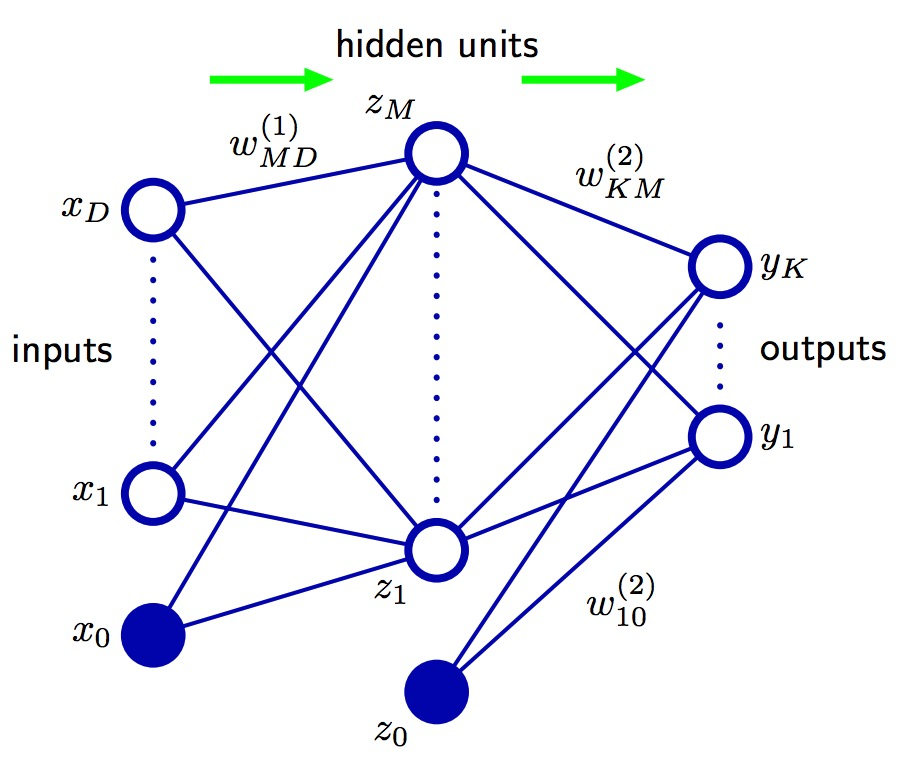
\includegraphics[width=0.7\linewidth]{images/ANN_representation.jpg}
  \caption{Network diagram for a two layer neural network. Image courtesy of \textcite{Bishop:2006}}
  \label{fig:ANN_representation}
\end{figure}

% Image found at page 228 in Bishop book: http://users.isr.ist.utl.pt/~wurmd/Livros/school/Bishop%20-%20Pattern%20Recognition%20And%20Machine%20Learning%20-%20Springer%20%202006.pdf

When feeding forward initially the data constitutes the input of the network. The input signal is equal to the dimensionality of the data. Forwarding the signal to the first layer a linear transformation is applied to the signal involving two parameters conclusive to the layer, weight and bias, thus transforming the signal. The transformed signal is sent through a activation function amplifying or reducing the signal based on its current value, producing a new output. The current output is then considered the input for a new set of weights and biases forwarding the signal repeatedly in the same manner until reaching the final layer. In the final layer the signal is converted to probabilities of each possible output of the network \parencite{Bishop:2006}.

Back propagation is where an ANN is tuning the wights and biases to produce sensible outputs in relation to the input. Feeding an input of training data forward an error can be computed from the difference between the received output probabilities and the expected output. The error is in turn propagated backwards tuning the parameters to produce the expected output instead. Repeating this process for all training data network increases its prediction accuracy \parencite{Bishop:2006}.

\subsection{Decision Trees}

Tree based methods involve stratifying or segmenting the predictor space into a number of simple regions. In order to make a prediction for a given observation, the mean or the mode of the training observations is used in the region to which it belongs. Since the set of splitting rules used
to segment the predictor space can be summarised in a tree, these types of approaches are known as decision tree (DT) methods \parencite{James:2014}.

DTs can be applied both to regression as well as classification problems. We focus on classification DTs as its the nature of the classification at hand in this report.

To growing a classification tree recursive
binary splitting is performed. The binary spilt is based on classification error rate on the training data. Since we plan classification to assign an observation in a given region to the most commonly occurring error rate class of training observations in that region, the classification error rate is simply the fraction of the training observations in that region that do not belong to the most common class \parencite{James:2014}.

\subsection{Naïve Bayes}

Naïve Bayes (NB) have beens studied since the 1950 and is a supervised, probabilistic machine learning classifier. It uses the maximum posterior which statistically determines the probability of a data point, x, belonging to a certain class, y, given the observed data points:

\[
P(y|x) = \frac{P(x|y)P(y)}{P(x)}
\]

This formula can be read as:

\[
Posterior = \frac{Prior * Likelihood}{Evidence}
\]

The name of the methods originates from the fact that the maximum posterior is calculated with help of the Bayes' Theorem and the method is naïve in the aspect of it assuming that all features in the data are independent form each other. \parencite{george2012}

skriv lite mer, förklara posterior?

\subsection{Support vector machines}

Support vector machines (SVM) where developed in the 1990s and are base on the simpler maximal margin classifier. The maximal margin classifier creates a hyperplane to separate the data points of different classes from each other. The margin is the smallest perpendicular distance from the plane to the a data point. As the name of the method suggests the goal is to find the plane with the largest margin given the data set \textcite{James:2014}.

\begin{figure}[ht!]
  \centering
  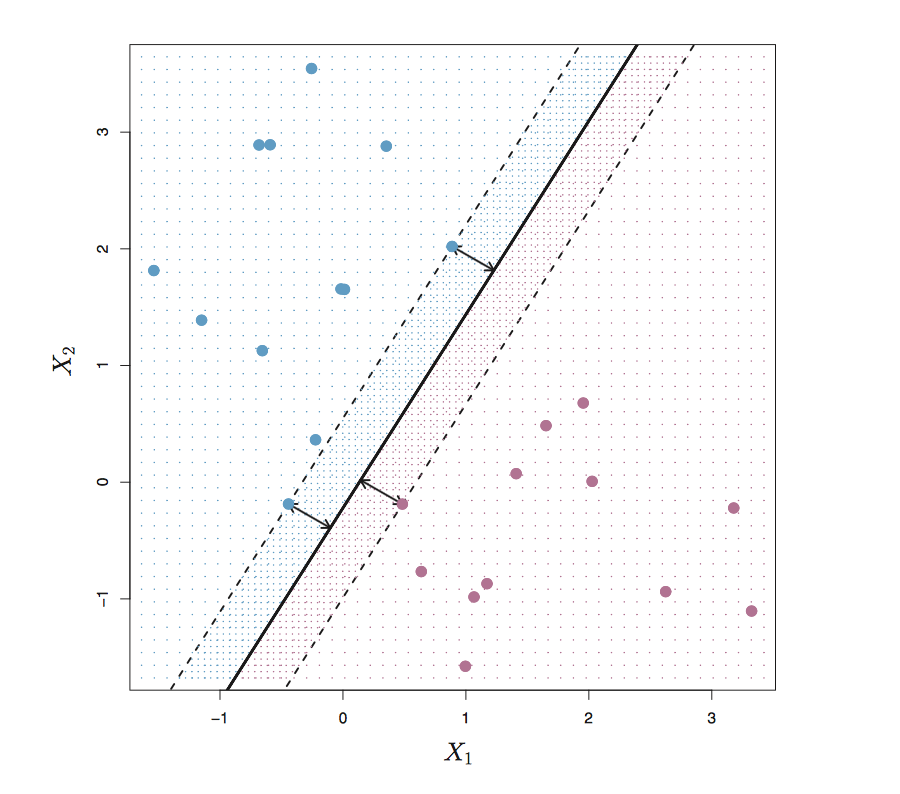
\includegraphics[width=0.7\linewidth]{images/Margin_SVM.png}
  \caption{Image of SVM margin. The red dots represent one class and the blue dots represent another class. The arrows indicates the maximal margin. Image courtesy of \textcite{James:2014}}
  \label{fig:SVM_Margin}
\end{figure}

The support vector classifier is an extension to the maximal margin method to try to create a method with greater robustness and better classification to most training observations. In order to achieve this goal an slack variable in introduced to allow points to be on the wrong side of the margin. Lastly, a SVM converts the support vector classifier from a liner separator as to  a non-liner separator of data points by using so called Kernels. The classifier can now separate more complex data sets with higher accuracy since its not limited to create linear hyperplanes \textcite{James:2014}.


\section{Feature Selection}

A feature is a variable that describes a data instance. A rectangular surface can be considered having two features, length and height. A rectangular volume three features, length, height and depth. More complex data instances such as a gene expression may have up to 60,000 features and such a complex feature space results in a much harder learning process. Thus one often wishes to select a subset of all available to reduce the dimensionality \parencite{guyon2003}.

The benefits of selecting a subset of all available features are manyfold, among other it facilitates data visualisation and data understanding, reduces the measurement and storage requirements and reduces training and utilisation times. In cases with thousands of features like the example with gene expressions it is essential to work with a subset of the data to produce reliable results. \parencite{guyon2003}.


\subsection{Filter methods}

Filter methods are considered as a preprocessing step. That means a filter method evaluate features before data is applied to a learning machine or even before a deciding on a classifier. The evaluation is performed by doing variable ranking by some score such as information gain. The score results in a ranking of the attributes and a subset can be selected in order of the ranking \parencite{guyon2003}.

There are both good and bad aspects of filter methods. The positive concerns that variable ranking makes filter methods very scalable and robust as the calculations only operated on as many variables as there are features and can be performed just once and tested on multiple classifiers making it very computational effective. On the other hand, a subset of features that by their own might be assessed an non informative by their own may in combination provide a lot of information to enable good learning \parencite{guyon2003}.


\subsection{Wrapper methods}

Wrapper methods differs a lot from filter methods. While filter methods evaluate the as a preprocessing independent of the classifier, wrapper does the opposite.

Wrappers utilise the learning machine of interest as a black box to score subsets of variable according to their predictive power \parencite{guyon2003}. The issue is as datasets become very large this method might be overly computational intense as finding the optimal subset is considered to be NP-hard \parencite{amaldi1998}.


\section{Computer Aided Diagnostics}

Machine learning techniques have been successfully applied to computer-aided diagnosis where it by a computerized procedure provides a second objective opinion for the assistance of medical image interpretation and diagnosis \parencite{li2007}, \parencite{ni2016}. To create a CAD system, samples with a diagnos is firstly gathered and stored and then used for learning. In the case of breast cancer diagnosis a radiologist put labels on a set of mammography scans. These include the diagnosis of the scan and possibly some attributes connected to the scan too, such as patients age or other conditions. These scans together with the labels can then be used to learn a hypothesis whether a undiagnosed sample is benign or malignant cancer \parencite{li2007}.


\section{Breast Cancer}

A study in Sweden by \textcite{tabar2001} found breast carcinoma mortality was reduced by 63\% after mammography was introduced. This clearly emphasize the benefits of screening which had resulted in a increased usage of the method to detect and diagnose breast cancer. The increasing demand for mammography image interpretation lead to a shortage of medical radiologist to perform this task and consequently non medical personnel supplement the mammography image interpretation \parencite{culpan2016}. As breast cancer still continues to be the leading cause of cancer mortality among women and more efficient diagnostics and pathology is high on demand the need of low-cost point-of-care is very much needed as stated by \textcite{martei2018}.

Fine needle aspiration (FNA) is a diagnostic tool to aspirate cell samples by sampling cells, staining them and examine under a microscope \parencite{FNA}. An example of such sample can be seen in \ref{fig:fna_nuclei}. The cell samples can be evaluated within 24 hours and the method is cost-effective and can be used as a preoperative tool for investigation of tumors. The method is also complication-free and has been widely used for the past 60 years.

\begin{figure}[ht!]
  \centering
  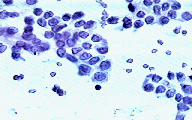
\includegraphics[]{images/fna_nuclei.png}
  \caption{A caption of a FNA sample as seen through a microscope. Image courtesy of Wisconsin University}
  \label{fig:fna_nuclei}
\end{figure}

% Image source: http://webcache.googleusercontent.com/search?q=cache:635J2rrIdWsJ:pages.cs.wisc.edu/~olvi/uwmp/cancer.html+&cd=1&hl=sv&ct=clnk&gl=se


\section{Related Work}

\textbf{ TBD: Make subsections where each section coves a specific topic. This can also be extended with almost another full page.}

The application of machine learning onto breast cancer classification is a well studied one. Since machine learning proved valuable empirical results breast cancer datasets have been widely used to assess the performance of a multitude of classification strategies and methods. [Insert ref. to early paper here].

Exhaustive studies for optimal Classifiers has been made as by \parencite{ramos2012} which tested 20,000 classification configurations to evaluated their ability to correctly classify malignant cancer. The achieved a result of 0.996 under the Receiver operating characteristic (ROC) curve.
% Add which method achieved the result above

With a foundation of well performing classifiers studies investigating more fine tuned approaches building upon earlier results were being made. \textcite{akin2011} demonstrated that ensemble learning can be used in CAD to improve the performance of rotation forest classifier. Using three different dataset and 30 classifying algorithms the average accuracy improved on all datasets by nearly 3\%.

\textcite{Abdel-Ilah2017} reported further improvements on ANNs by investigating the optimal number of hidden layers and neurons for a feed forward back propagation network. The highest accuracy acheived was 98\% using 3 hidden layers and 21 neurons with three distinct transfer functions.

\textcite{akay2009} investigated the performance of classification of a SVM with a RBF kernel using feature selection, filtering by F-score. They achieved a classification accuracy of 99.51\% which accordingly was among the highest scores recorded by then (2007).

\textcite{karabulut2012} made a comparative study on the effect of feature selection on classification accuracy and found up to 15.55\% improvement on classification rates. The study used only filter algorithms for feature selection, among those were both information and Chi-square. The study applied the selected features on three classification methods, Naive Bayes, Artificial Neural Network as Multilayer Perceptron, and J48 decision tree classifier on 15 different datasets including WBCD.

Building upon this foundation of work our study seeks to complete the field by providing further investigation of unreported selection methods such as SBS and SFS and review their performance on a combination of classifiers from the previous research presented here.
